\chapter{Results}

\section{Linear Baseline Model}

First a simple linear model was trained to establish a baseline accuracy.
Figure~\ref{linear_loss} shows the test and training loss for the linear model.

\begin{figure}
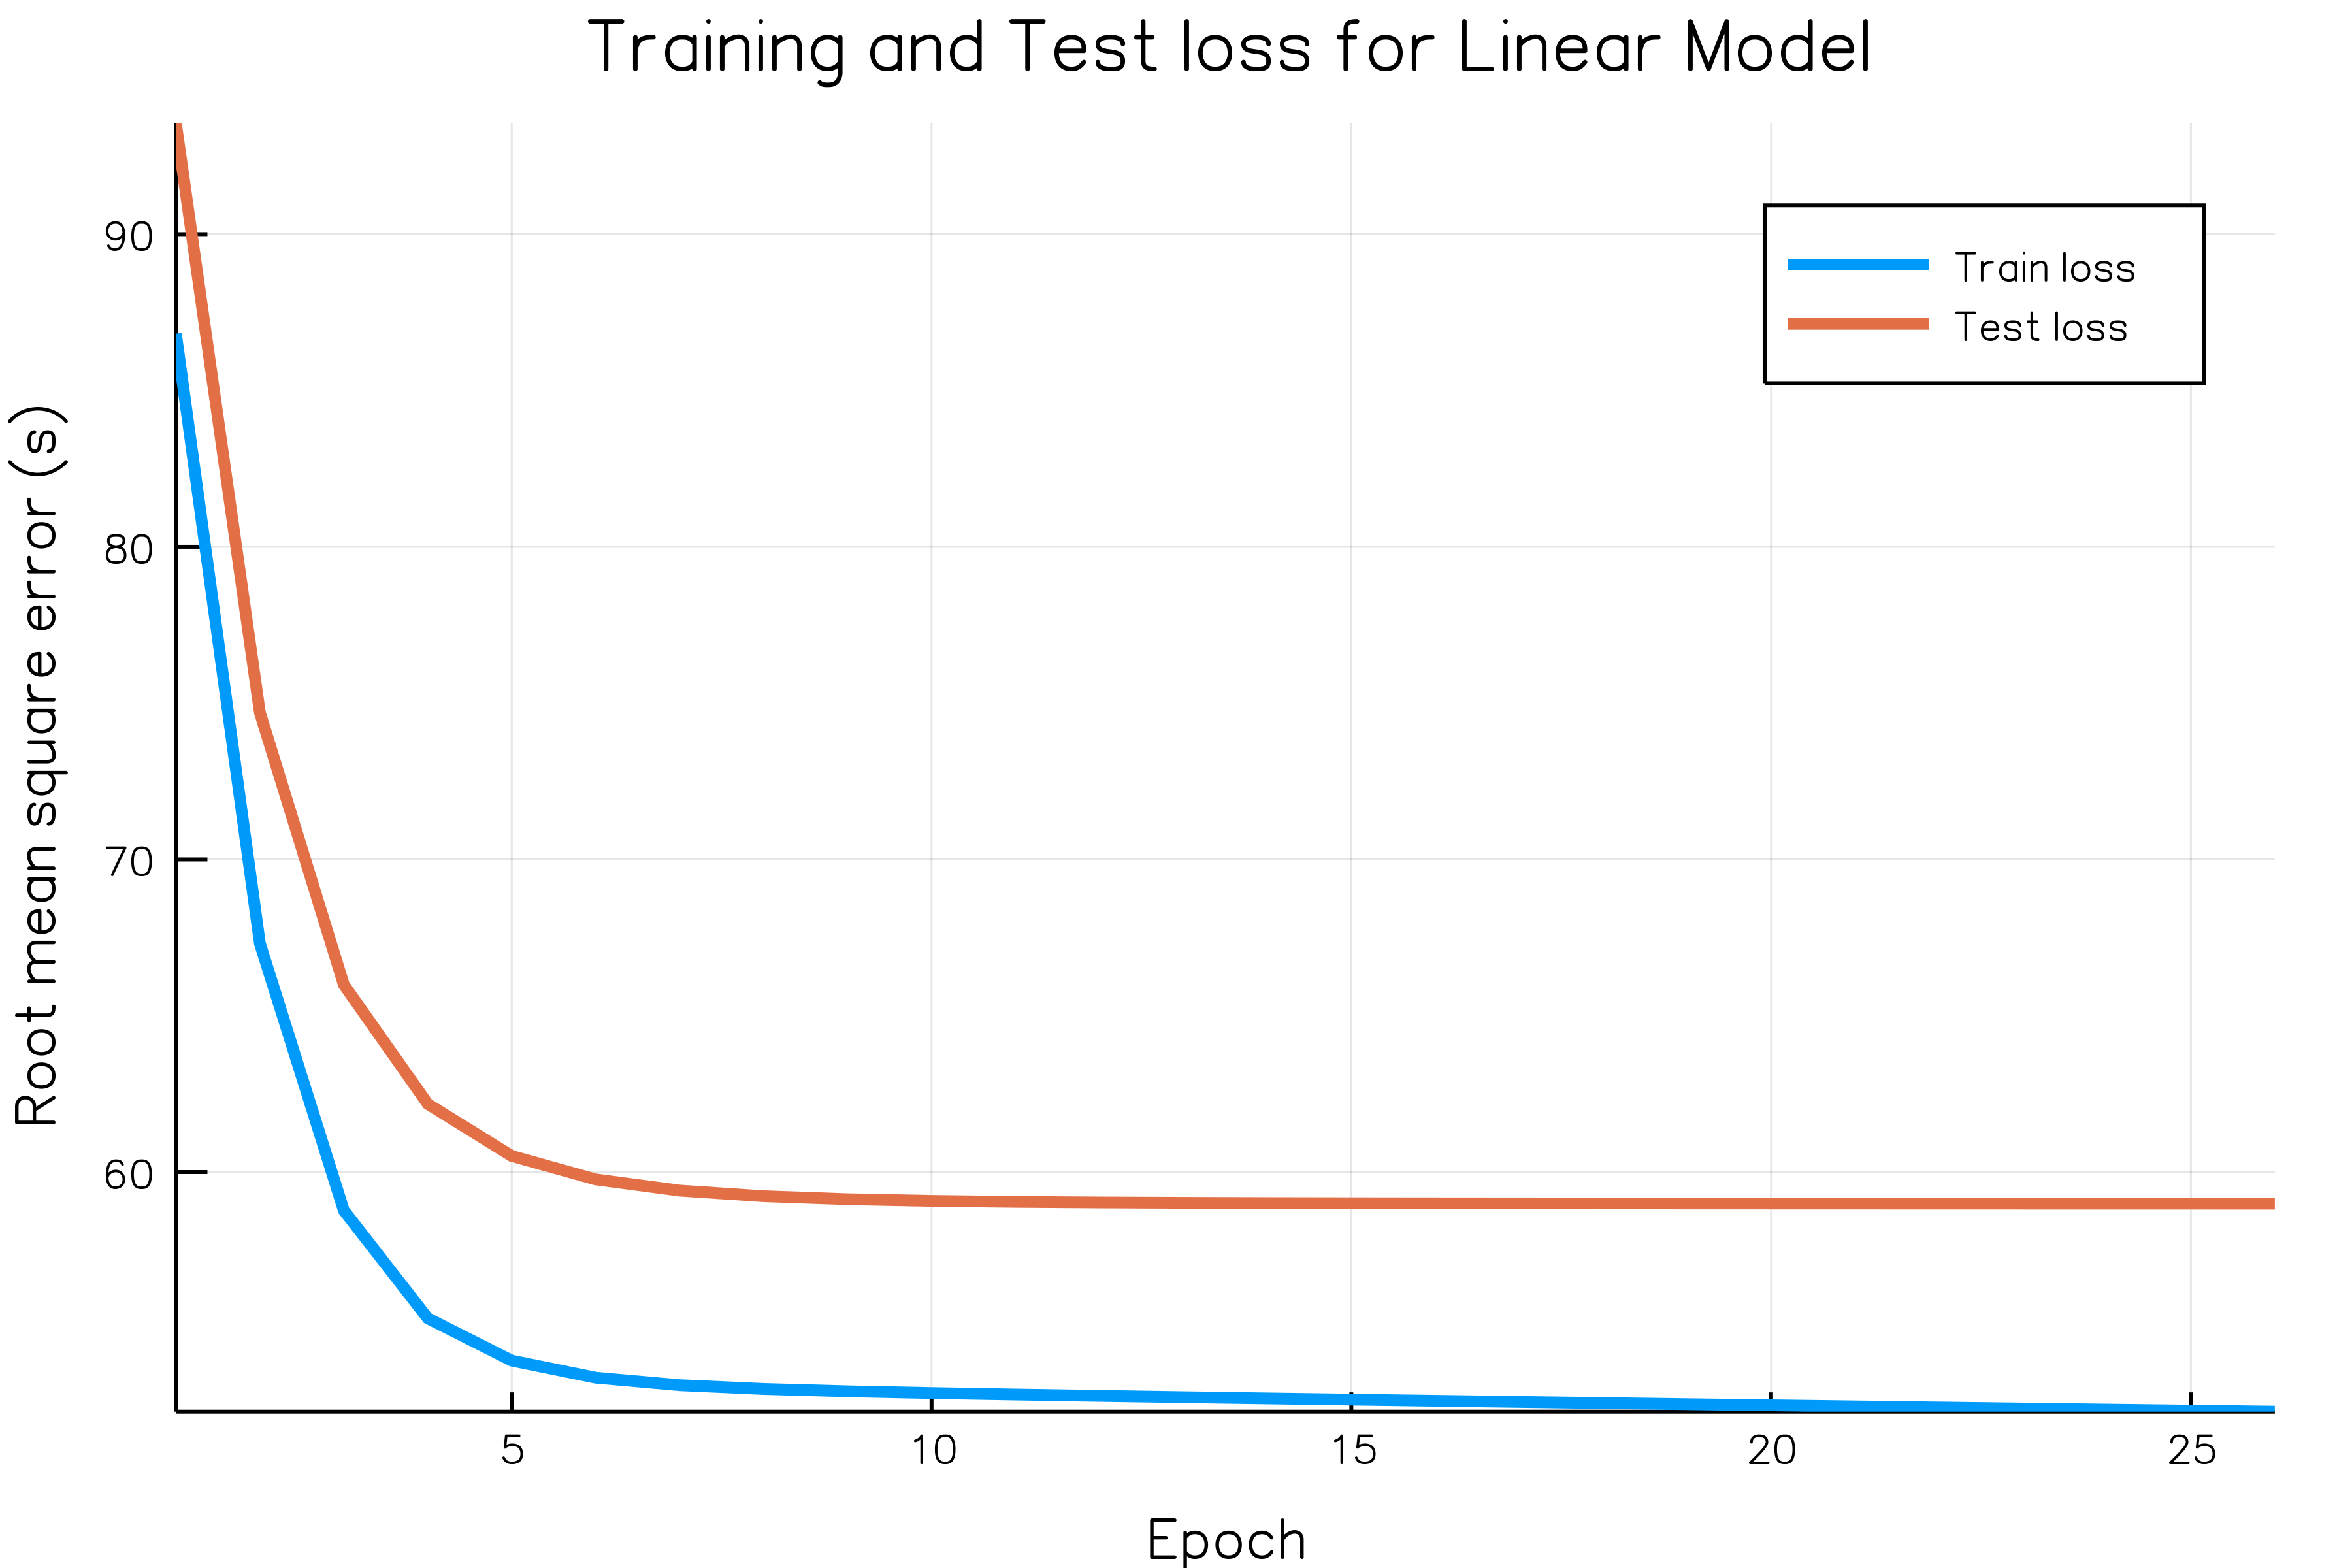
\includegraphics[width=\linewidth]{images/linear_loss.png}
%\vspace{2.4in}
\caption{Loss for linear model (lower is better). The plot shows characteristic overfitting, with a test loss baseline just under 60 seconds.}
\label{linear_loss}
\end{figure}
\clearpage
\newpage

The loss curve is smooth, and follows our expectation for the training loss to be slightly better than the test loss.
Furthermore, this model allows us to establish the baseline accuracy of ~60 seconds for test RMSE.
The further models will be compared against the linear model.

\section{MLP}

The next model trained was the multilayer perceptron.
The MLP has much more expressive power than the linear model, so one would expect that the training loss will be significantly lower.
However the high variance of the model can lead to poor performance on the test set.
Figure~\ref{mlp_loss} shows the loss curves for the MLP model.
As expected, the training loss is significantly lower, with a RMSE of around 30 seconds.
The test loss is significantly higher, but still better than the linear model.
This shows that the model was able to capture more of the variability in the data.

\begin{figure}
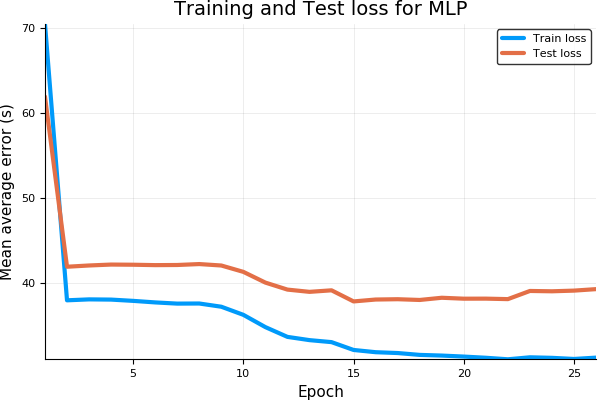
\includegraphics[width=\linewidth]{images/mlp_loss.png}
%\vspace{2.4in}
\caption{Loss for MLP model (lower is better). The MLP can capture more of the variation in outputs than the linear model.}
\label{mlp_loss}
\end{figure}
\clearpage
\newpage

\section{CNN}

Figure~\ref{cnn_loss} shows the loss curves for the CNN model.
The CNN model improves slightly on the MLP model.
It achieves a test RMSE of around 37 seconds.
The CNN model is significantly larger, and takes longer to train than the MLP.
An interesting observation is that the loss curve for training starts increasing after around 10 iterations.
The larger model seems to have some difficulty with convergence.
The model is trained until the validation accuracy stops decreasing, which occurs at around 25 epochs.

\begin{figure}
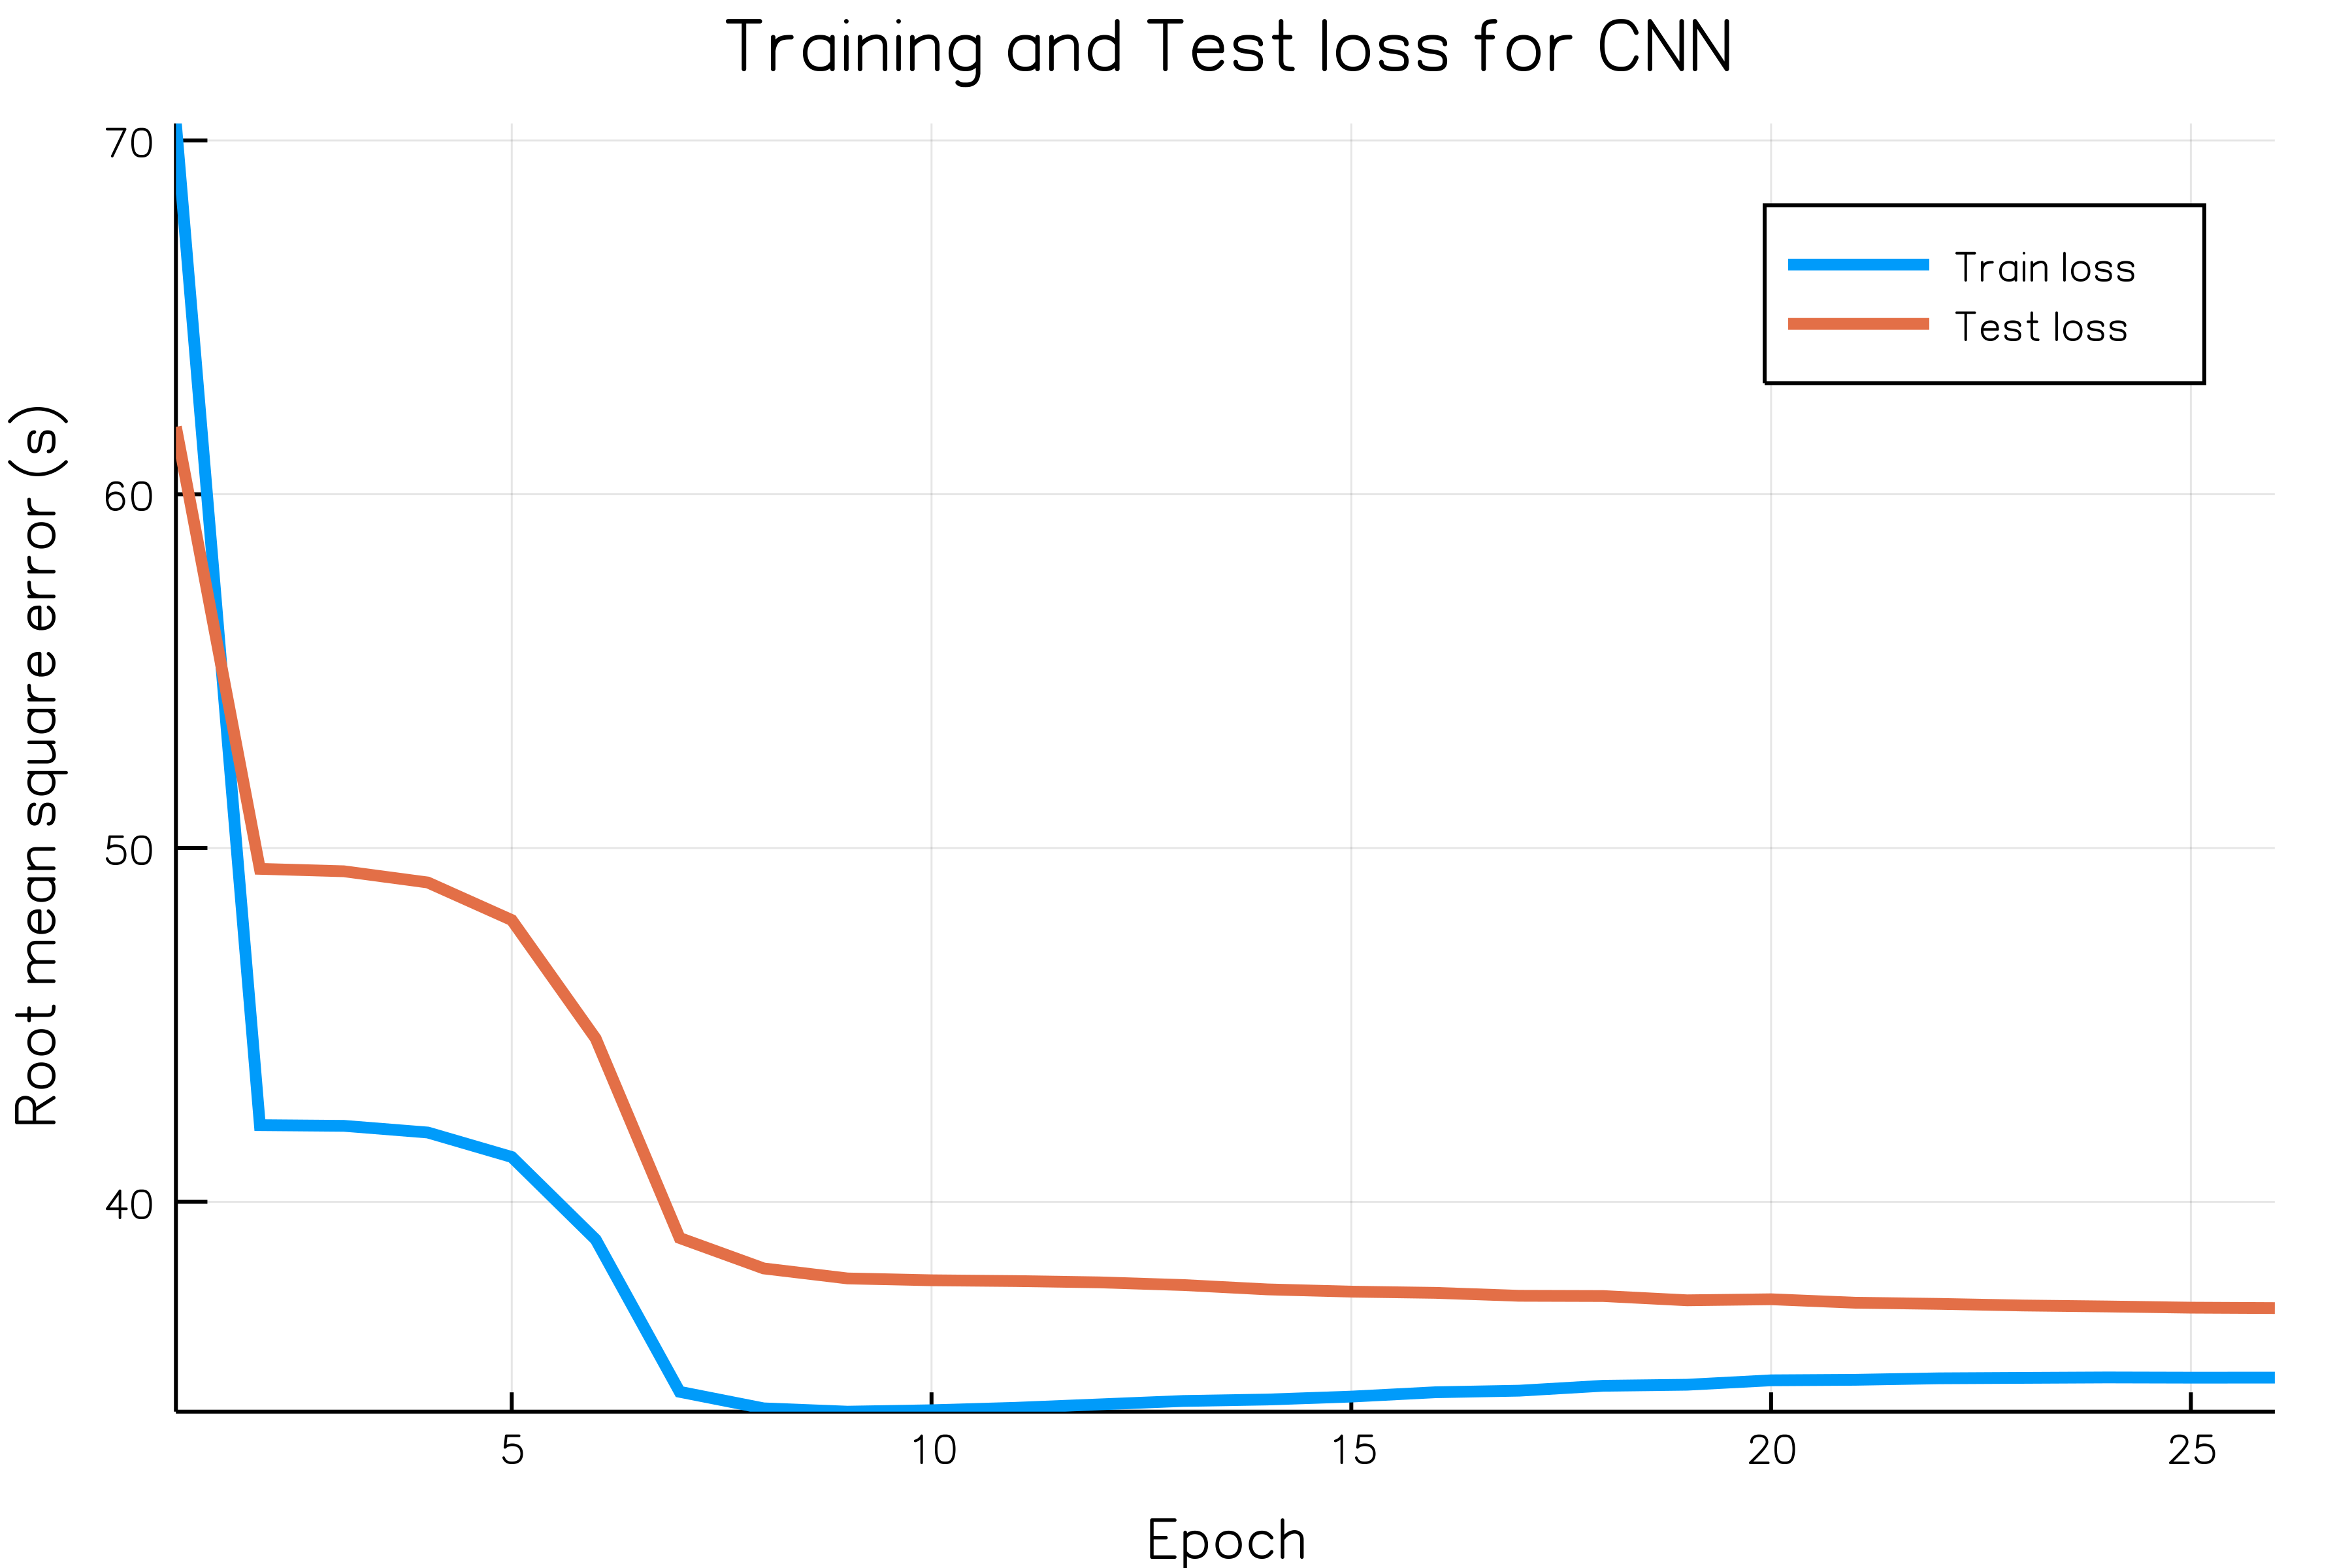
\includegraphics[width=\linewidth]{images/cnn_loss.png}
%\vspace{2.4in}
\caption{Loss for CNN model (lower is better). The CNN improves upon the accuracy of the MLP.}
\label{cnn_loss}
\end{figure}
\clearpage
\newpage

\section{RNN}

The final model trained was an RNN.
RNNs take significantly longer to train due to the back propagation through time algorithm requiring an entire sequence to be feed through the network for each update.
In this case, the prediction optimization for future stops was optimized rather than the entire sequence.

RNNs are considered more difficult to train than other forms of models because of the exploding/vanishing gradient problem \cite{pascanu2013difficulty}.
During back propagation through time, the signal to train the network passes through the neural network several times.
If the magnitude of the gradient does not stay relatively constant between time steps, the gradient and exponentially blow up or shrink.
This reduces the quality of gradients and makes training the networks more difficult.
The same effect occurs in large feed forward networks with many layers, such at deep CNNs.
In feed forward networks, this effect is mitigated with batch normalization\cite{ioffe2015batch}.
For RNNs, sequence to sequence mapping does not have as much of an issue with exploding and vanishing gradient, because signal is added to the gradient at each timestep.
However for regression problems, the signal is only received at the end, and then has to be propagated back over the network several times.
For this reason, the size of RNNs for regression tasks is limited.

Figure~\ref{rnn_loss} shows the loss curves for training this model.
The loss curves are much noisier than the other models.
However, the model converges eventually to just under 30 seconds for training and just over 30 seconds for test.
This represents the best overall loss across all of the models.

\begin{figure}
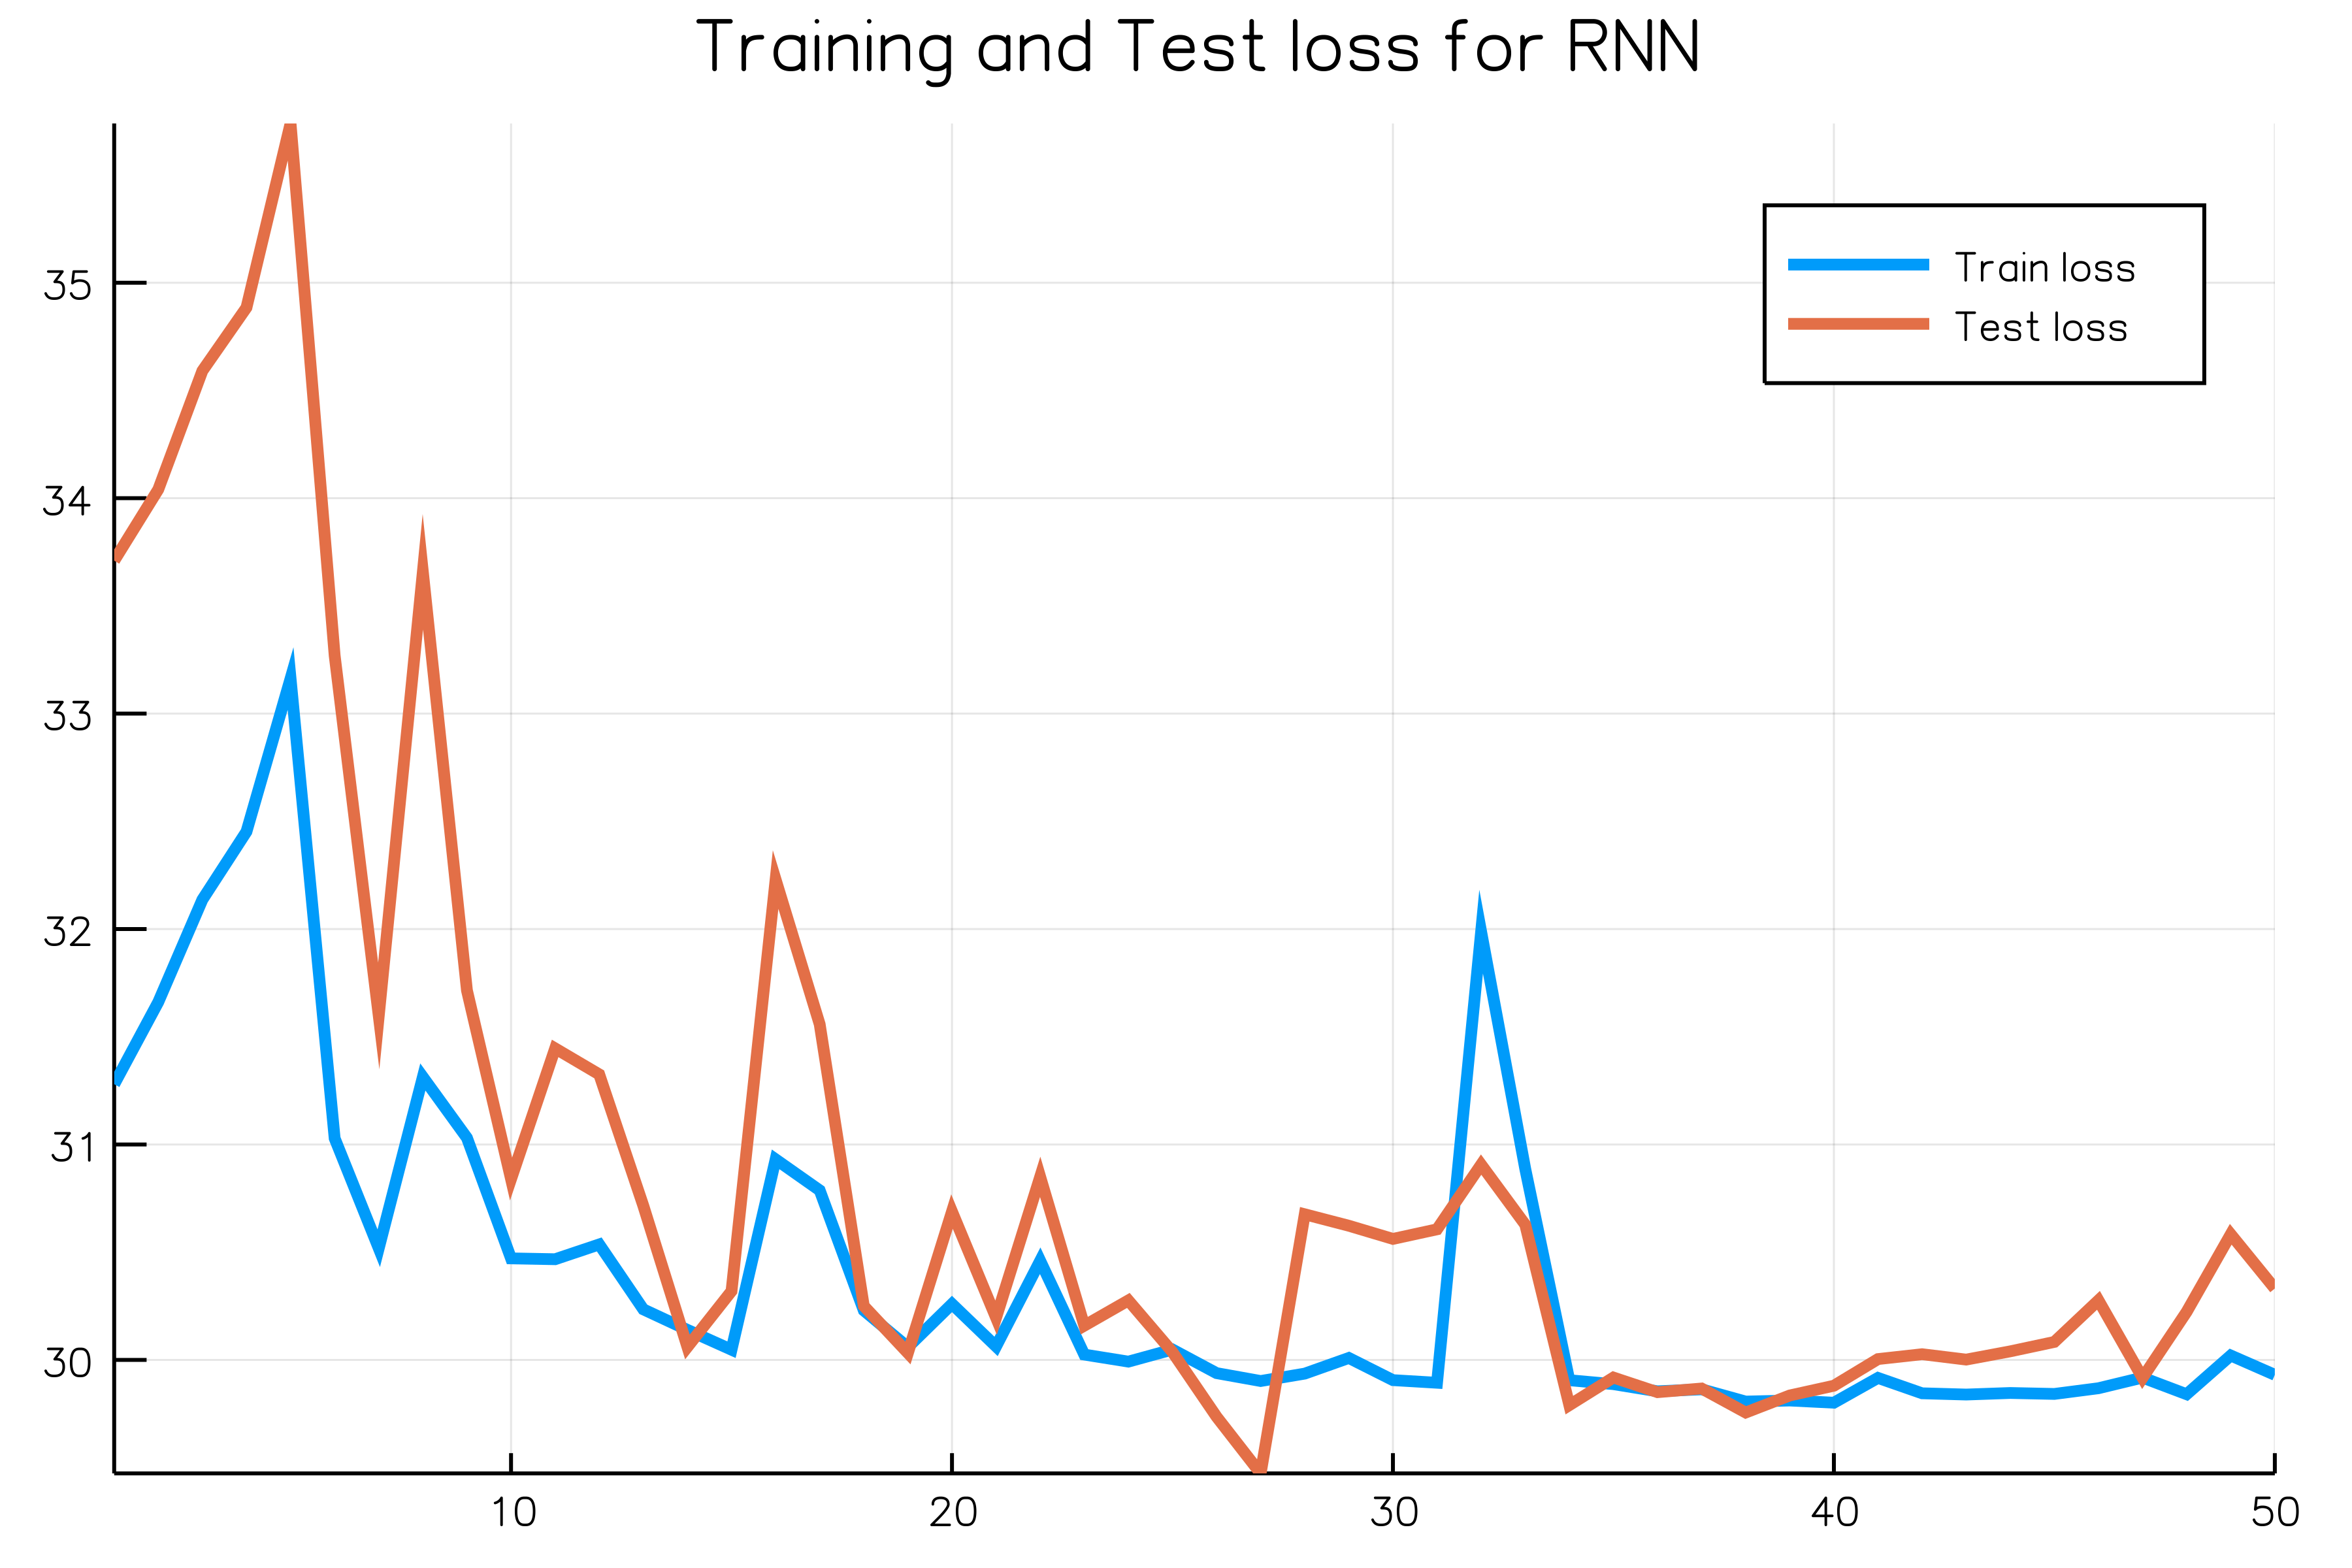
\includegraphics[width=\linewidth]{images/rnn_loss.png}
%\vspace{2.4in}
\caption{Loss for RNN model (lower is better). The RNN achieves the lowest overall loss.}
\label{rnn_loss}
\end{figure}
\clearpage
\newpage


\begin{table}
\caption{Root mean square error for all models}
\label{loss_table}
\begin{center}
\begin{tabular}{|l|l|l|l|l|}\hline
      & Linear & MLP & CNN & RNN \\\hline
Train & 59.2 & 31.2 & 35.0 & 29.8 \\\hline
Test  & 54.3 & 39.9 & 37.5 & 30.4 \\\hline
\end{tabular}
\end{center}
\end{table}

Table~\ref{loss_table} summarizes the final loss values for all of the models, and table~\ref{r2_table} summarizes the $R^2$ score for each of the models.

\begin{table}
\caption{$R^2$ score for all models}
\label{r2_table}
\begin{center}
\begin{tabular}{|l|l|l|l|l|}\hline
      & Linear & MLP    & CNN   & RNN   \\\hline
Train & 0.5673 & 0.8798 & 0.8488 & 0.8904 \\\hline
Test  & 0.636  & 0.8035 & 0.8264 & 0.8859 \\\hline
\end{tabular}
\end{center}
\end{table}
